% TEMPLATE for Usenix papers, specifically to meet requirements of
%  USENIX '05
% originally a template for producing IEEE-format articles using LaTeX.
%   written by Matthew Ward, CS Department, Worcester Polytechnic Institute.
% adapted by David Beazley for his excellent SWIG paper in Proceedings,
%   Tcl 96
% turned into a smartass generic template by De Clarke, with thanks to
%   both the above pioneers
% use at your own risk.  Complaints to /dev/null.
% make it two column with no page numbering, default is 10 point

% Munged by Fred Douglis <douglis@research.att.com> 10/97 to separate
% the .sty file from the LaTeX source template, so that people can
% more easily include the .sty file into an existing document.  Also
% changed to more closely follow the style guidelines as represented
% by the Word sample file. 

% Note that since 2010, USENIX does not require endnotes. If you want
% foot of page notes, don't include the endnotes package in the 
% usepackage command, below.

% This version uses the latex2e styles, not the very ancient 2.09 stuff.
\documentclass[letterpaper,twocolumn,10pt]{article}
\usepackage{usenix,epsfig,endnotes}
\usepackage[T1]{fontenc}
\usepackage{epstopdf}
\usepackage{enumitem}
\begin{document}

%don't want date printed
\date{}

%make title bold and 14 pt font (Latex default is non-bold, 16 pt)
\title{\Large \bf Building a Modular ROS Network for the Raven II}

%for single author (just remove % characters)
\author{
{\rm Troy\ Sankey}\\
University of California Los Angeles
\and
{\rm Qu\ (Jackie)\ Jin}\\
University of California Los Angeles
\and
{\rm Jonathan\ Chan}\\
University of California Los Angeles
} % end author


\twocolumn[
  \begin{@twocolumnfalse}
    \maketitle
    \vspace{5cm}
    \hfill
    \begin{minipage}{0.8\linewidth}
      \begin{abstract}

The Raven II is a 7-DOF cable-actuated surgical robot designed for
minimally invasive and remote surgery. It utilizes Robot Operating
System (ROS), a collection of software modules specially made for
developing robot applications. Many features of ROS could be
beneficial to the the Raven, but are inaccessible due to current
code's limited use of ROS constructs. Our team has integrated ROS into
the Raven II which will bring better support for generic control,
image processing, basic automation, and overall cleaner and more
reliable code. This report covers the benefits of a ROS-centric system
and details on how we have integrated ROS into the existing code.

      \end{abstract}
    \end{minipage}
    \hfill
  \end{@twocolumnfalse}
]

\thispagestyle{empty} % we don't want a page number on the title page
\clearpage % end the title page
\setcounter{page}{1} % we want the page numbering to start here

\section{Introduction}
The Raven II surgical robotic arm was designed by the BioRobotics
Laboratory (BRL) at the University of Washington, and one copy of the
robot was given to the Center for Advanced Surgical and Interventional
Technology (CASIT) at the University of California Los Angeles to help
study and improve.

The Raven is designed to enhance remote surgical operations, and 
minimally invasive surgery (MIS). BRL achieved this feat by using the 
Omni haptic devices to remotely control the Raven. However, this is 
only the first step in improving robotic surgery in MIS.

Ultimately, we plan to develop three areas of Raven function: novel
controllers, generic automation, and image recognition. Novel
controllers are beneficial because the Omni devices are not intuitive
to use.  Furthermore, because the Raven is software controlled, we can
use software to enhance the surgeon's capabilities. Two main areas we
aim to develop are generic automation, and image recognition.
Automation includes many features. In the near future, we plan to
focus on the ability to define and record \emph{paths} that the
robotic arm has taken. This would allow for training the Raven to
perform certain tasks, like automated suturing, or automatically
positioning the robotic arms in a particular configuration. Another
feature of automation would be \emph{no-fly zones}---zones where the
raven is prohibited from moving in to (e.g. sensitive tissues).  Image
recognition is also a software capability that could enhance MIS by
improving automation. The camera and software analysis provides a
closed loop feedback system to the automated ability, thus improving
any automated tasks.

Unfortunately, when our team analyzed the code base of the Raven 
project, we found it difficult to develop on. The problem was the lack 
of modularity in the system. Each subsystem was tightly coupled with 
other subsystems, requiring very in depth knowledge of the entire 
code base to be able to add features. With such a interdependent 
system, it was difficult to take one part (e.g. the controller) and 
enhance it, without requiring a large fix, or breaking some other 
subsystem. In addition, the lack of modularity decreases code 
shareability. This unessecary complexity hinders not only our 
development of new features, but also the development by any other 
group.

To tackle this problem, we restructure the code base around the Robot
Operating System (ROS) framework. It is highly distributed, and 
provides many constructs for hardware abstraction, package management, 
and functional libraries designed for robotic systems. Thus the 
revamped Raven system we are developing aims to utilizes the the full 
power  of ROS to keep the code base modular, so that features can be 
easily added. This has been the bulk of this past quarter's work.

\section{Requirements}

\subsection{Understanding the Original (BRL) Raven code}

\begin{figure}[h]
  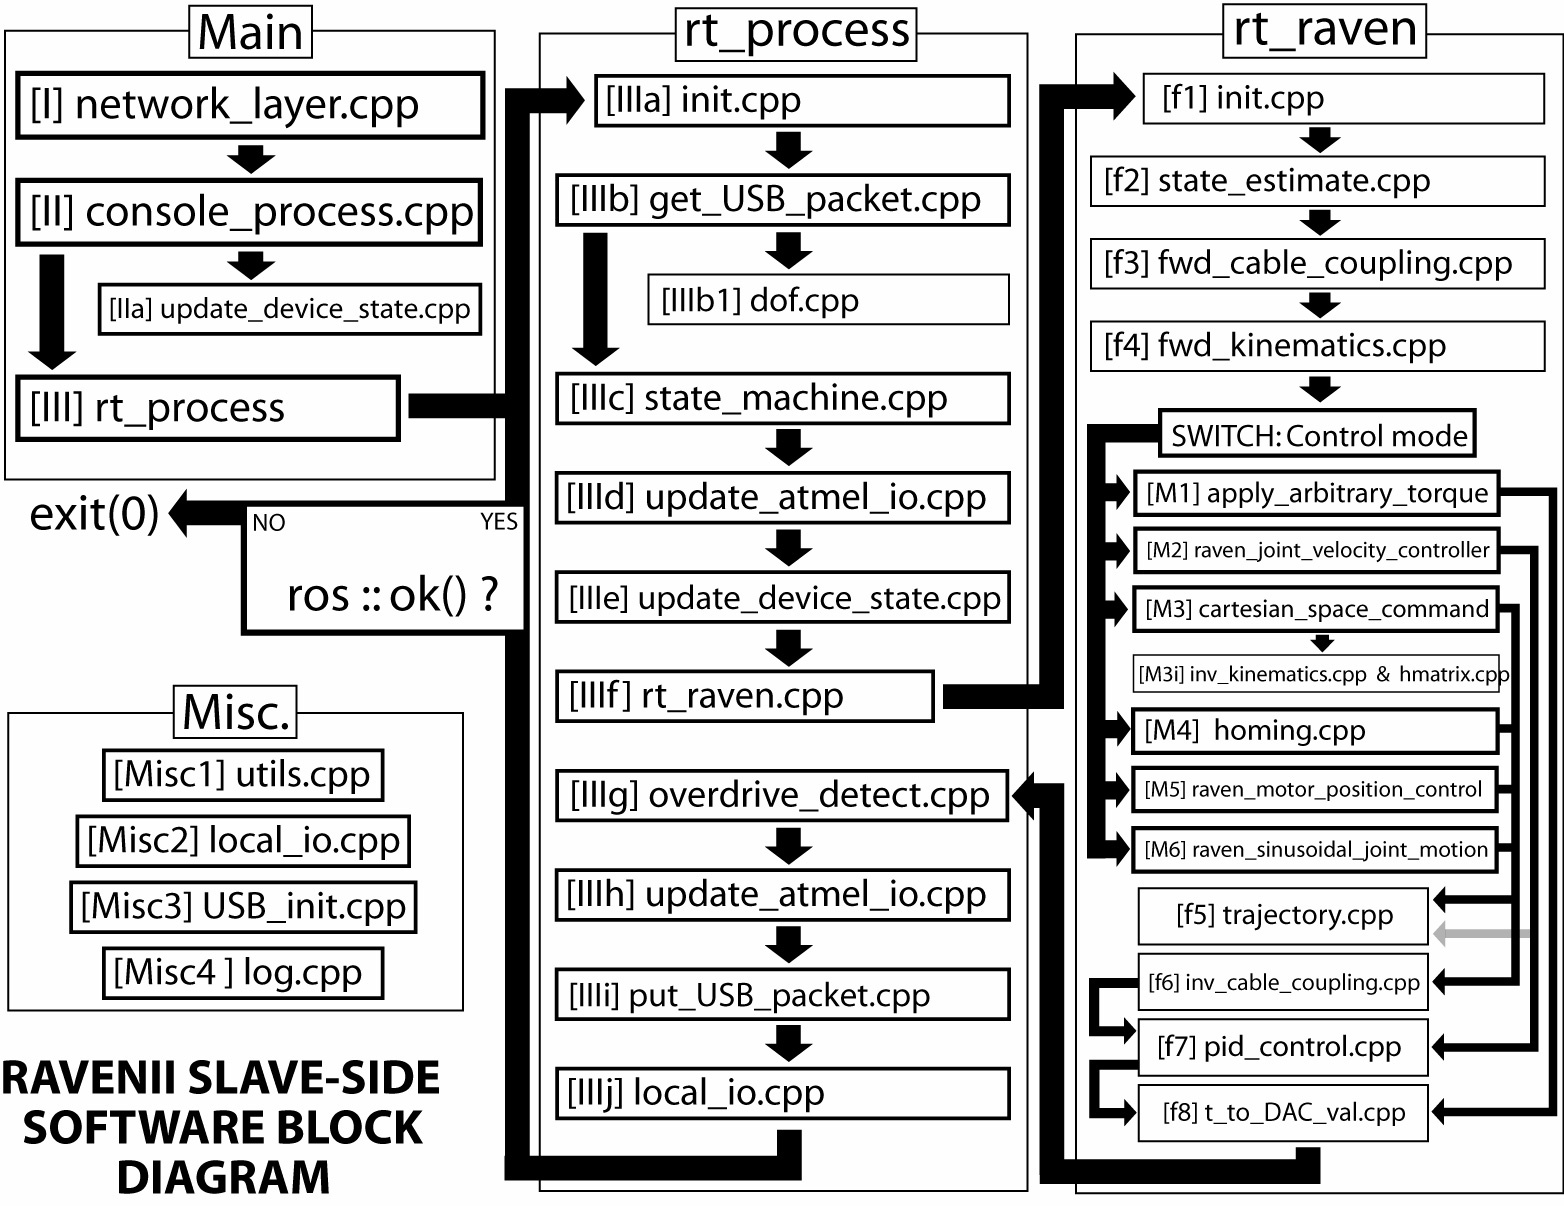
\includegraphics[scale=0.33]{RavenII_Block_Diagram.jpg}
  \caption{Raven II Call Diagram}
  \label{fig:block_diagram}
\end{figure}

The structure of the current raven system is straightfoward. At the
highest level, there is a master node and a slave node. The master
interprets the position and orientation of two Phantom Omni haptic
controllers (for both arms), translates them into a differential
position and orientation, then transmits that to the slave. The slave
will accumulate the differential pose\footnote{in robotics, \emph{pose}
  is the combination of position and orientation} into an absolute
pose, or goal pose, then attempt to reach the goal pose.

The master node makes use of the Phantom Omni API for determining
differential poses and grasp values for each arm. There is also a
pedal connected to the master computer to determine whether the
operator wants to engage or disengage the robot. During each iteration
it encapsulates all that data in UDP packets and sends them to the
slave node.

\vspace{0.5em}
\noindent
The slave code spawns three threads:
\begin{itemize}[noitemsep]
  \item networking
  \item control (e.g. IK, USB I/O)
  \item console I/O
\end{itemize}

The \emph{networking thread} listens for UDP packets from the master
node, then accumulates the differential pose into an absolute pose
that represents the desired pose. The \emph{control thread} is a
realtime thread that, at a fixed interval, retrieves the latest
desired pose, calculates torques for each motor, and applies those
torques (this process is called PID control). The control thread
encapsulates what is referred to as the \emph{control loop}, and can
be seen in the source file \texttt{rt\_process\_preempt.c}. The
\emph{console I/O} thread is used for initializing the robot and
printing status updates.

The complexity of the system is in the slave system. It is the bulk 
of the Raven code, and is highly interdependent. Thus, it is difficult 
to either make the slave perform any new tasks (by editing the slave 
code), or creating an arbitrary master or controller, because the 
slave code only knows how to listen to an Omni controlled master.

\subsection{Modularity from ROS}

Many components in the Raven code required specific knowledge of
several other components. In a fully modular system, each component
would not require such information, but would compensate in
functionality by adding slightly more components that each do slightly
simpler, more general tasks. In a well designed modular system, each
component's input and output is clearly defined.

For example, the UDP packets being sent from the master to the slave
need to be manually sequenced---if, at the slave (recieving) node, the
differential poses are not processed in-order, then the accumulated
absolute pose might sometimes have a meaningless value. In a modular
system, there may be an additional \emph{sequencer} module that
handles one simple task: sequencing packets in an unreliable
link. Incidentally, ROS provides an alternative transport layer, 
UDPROS, that fills the role of a sequencer module.

The key to attaining modularity from ROS is to make use of its nodes, 
and interfaces between nodes. Each subsystem has a task, and can be 
considered a node. Its code can be independent of that of other nodes. 
ROS provides interfacing between nodes with \emph{topics} and 
\emph{services}. These important constructs allow nodes to work 
independently for the most part, and when they need to communicate, 
there exists a standard messaging mechanism.

By breaking up tasks so that each node is responsible for one task, 
it is easy to add features. For instance, the node that is designed 
to receive TCP packets from the master can be easily replaced with 
a better node that uses UDPROS to receive UDP packets from the master. 
Since the node is independent of other nodes in the system, 
functionality of other parts will not be compromised.


\subsection{Novel controllers}
We would like to pursue developing novel controllers for the Raven
because a variety of technologies offer much better functionality than
the Omni devices. Such technologies include laparoscopic tools, motion
sensors, and tactile/haptic feedback devices that can enhance MIS in
ways that the Omni devices can not.  The default Omni devices have
limitations that make them difficult to use. Surgeons who attempted to
perform tasks with the Omnis found their narrow range of motion to be
a problem. One often reached the maximum bound of the Omni device,
before the Raven's end effector was in the correct position. To
continue the path to the desired position, the user had to release
control of the Raven, re-position the Omni devices back within range,
before continuing their path.

Our goal is to develop alternative controllers that allow surgeons to
focus on the surgery, and be unhindered by the controller. The ideal
controller would give surgeons the same dexterity as their trained
hands, and the haptic and tactile feedback that they are used to with
their sense of touch.

Many controllers designed to be more intuitive and dexterous already
exist. For instance, there is work in CASIT to interface the Raven
with laparoscopic graspers. Surgeons familiar with laparoscopic tools
will be able to more easily adapt to using the Raven.

Furthermore, motion sensors like the Leap Motion and the Microsoft
Kinect can track a user's hands and fingertips without the use of any
tools attached to the user. This offers even more intuitive hand
motion control. The major advantage of these controllers is the
increased sensitivity to the surgeon's finger tips. After a surgeon
performs the gross motion of moving the end effectors into a
particular position with his/her arms, they could then scale down the
sensitivity of the controller, and then focus on detailed tasks with
their fingers and wrist (e.g. suturing).

Another aspect of intuitive control is haptic and tactile feedback. A
Raven fitted with force sensors could provide a valuable tactile
feedback about its tool tip. Also, since the Raven performs
Proportional Integral Derivative (PID) control to determine motor
voltages, it is also aware of the amount of force necessary to move
its joints into a particular position. Thus, it has haptic information
as well that could be conveyed to an advanced controller.

A variety of controllers can be customized to enhance laparoscopic
surgery. These are only a few ideas on how to make enhancements with
existing technology. The Raven is a useful platform to research such
tools. Thus, it is important to make it easy for developers to create
novel controllers, without having to worry about cumbersome details
about the Raven system, while still being able to take full advantage
of the Raven's capabilities.

\subsection{Automation}
The Raven should be aware of the position of its arms in the real 
world, so that it can choose which paths to follow, and which paths 
to avoid.

If the Raven can understand intuitive positionings, like Cartesian 
coordinates, then a human can both define paths for the Raven to move 
in, and also no-fly zones, bounding its movements. 

\subsection{Image recognition}
Image recognition systems that make use of a camera to recognize the
context which its end-effectors are in can improve the Raven's
automation accuracy. We may want the Raven to infer its pose or the
positions of organs, so it can make decisions depending on the
situation. For instance, the system can learn to recognize a moving
organ, and ensure that the its end-effector is always kept at a 2 mm
distance from the surface of the organ. In general, 3D boundaries may
be constructed from 2D video which can be used to define no-fly zone.

Additional sensors may be used to detect distance, so a depth map
can be constructed and overlayed on the surgeon's viewing screen to
help complement the surgeon's lack of depth perception.

\section{Design}

\begin{figure*}[t]
  \begin{center}
    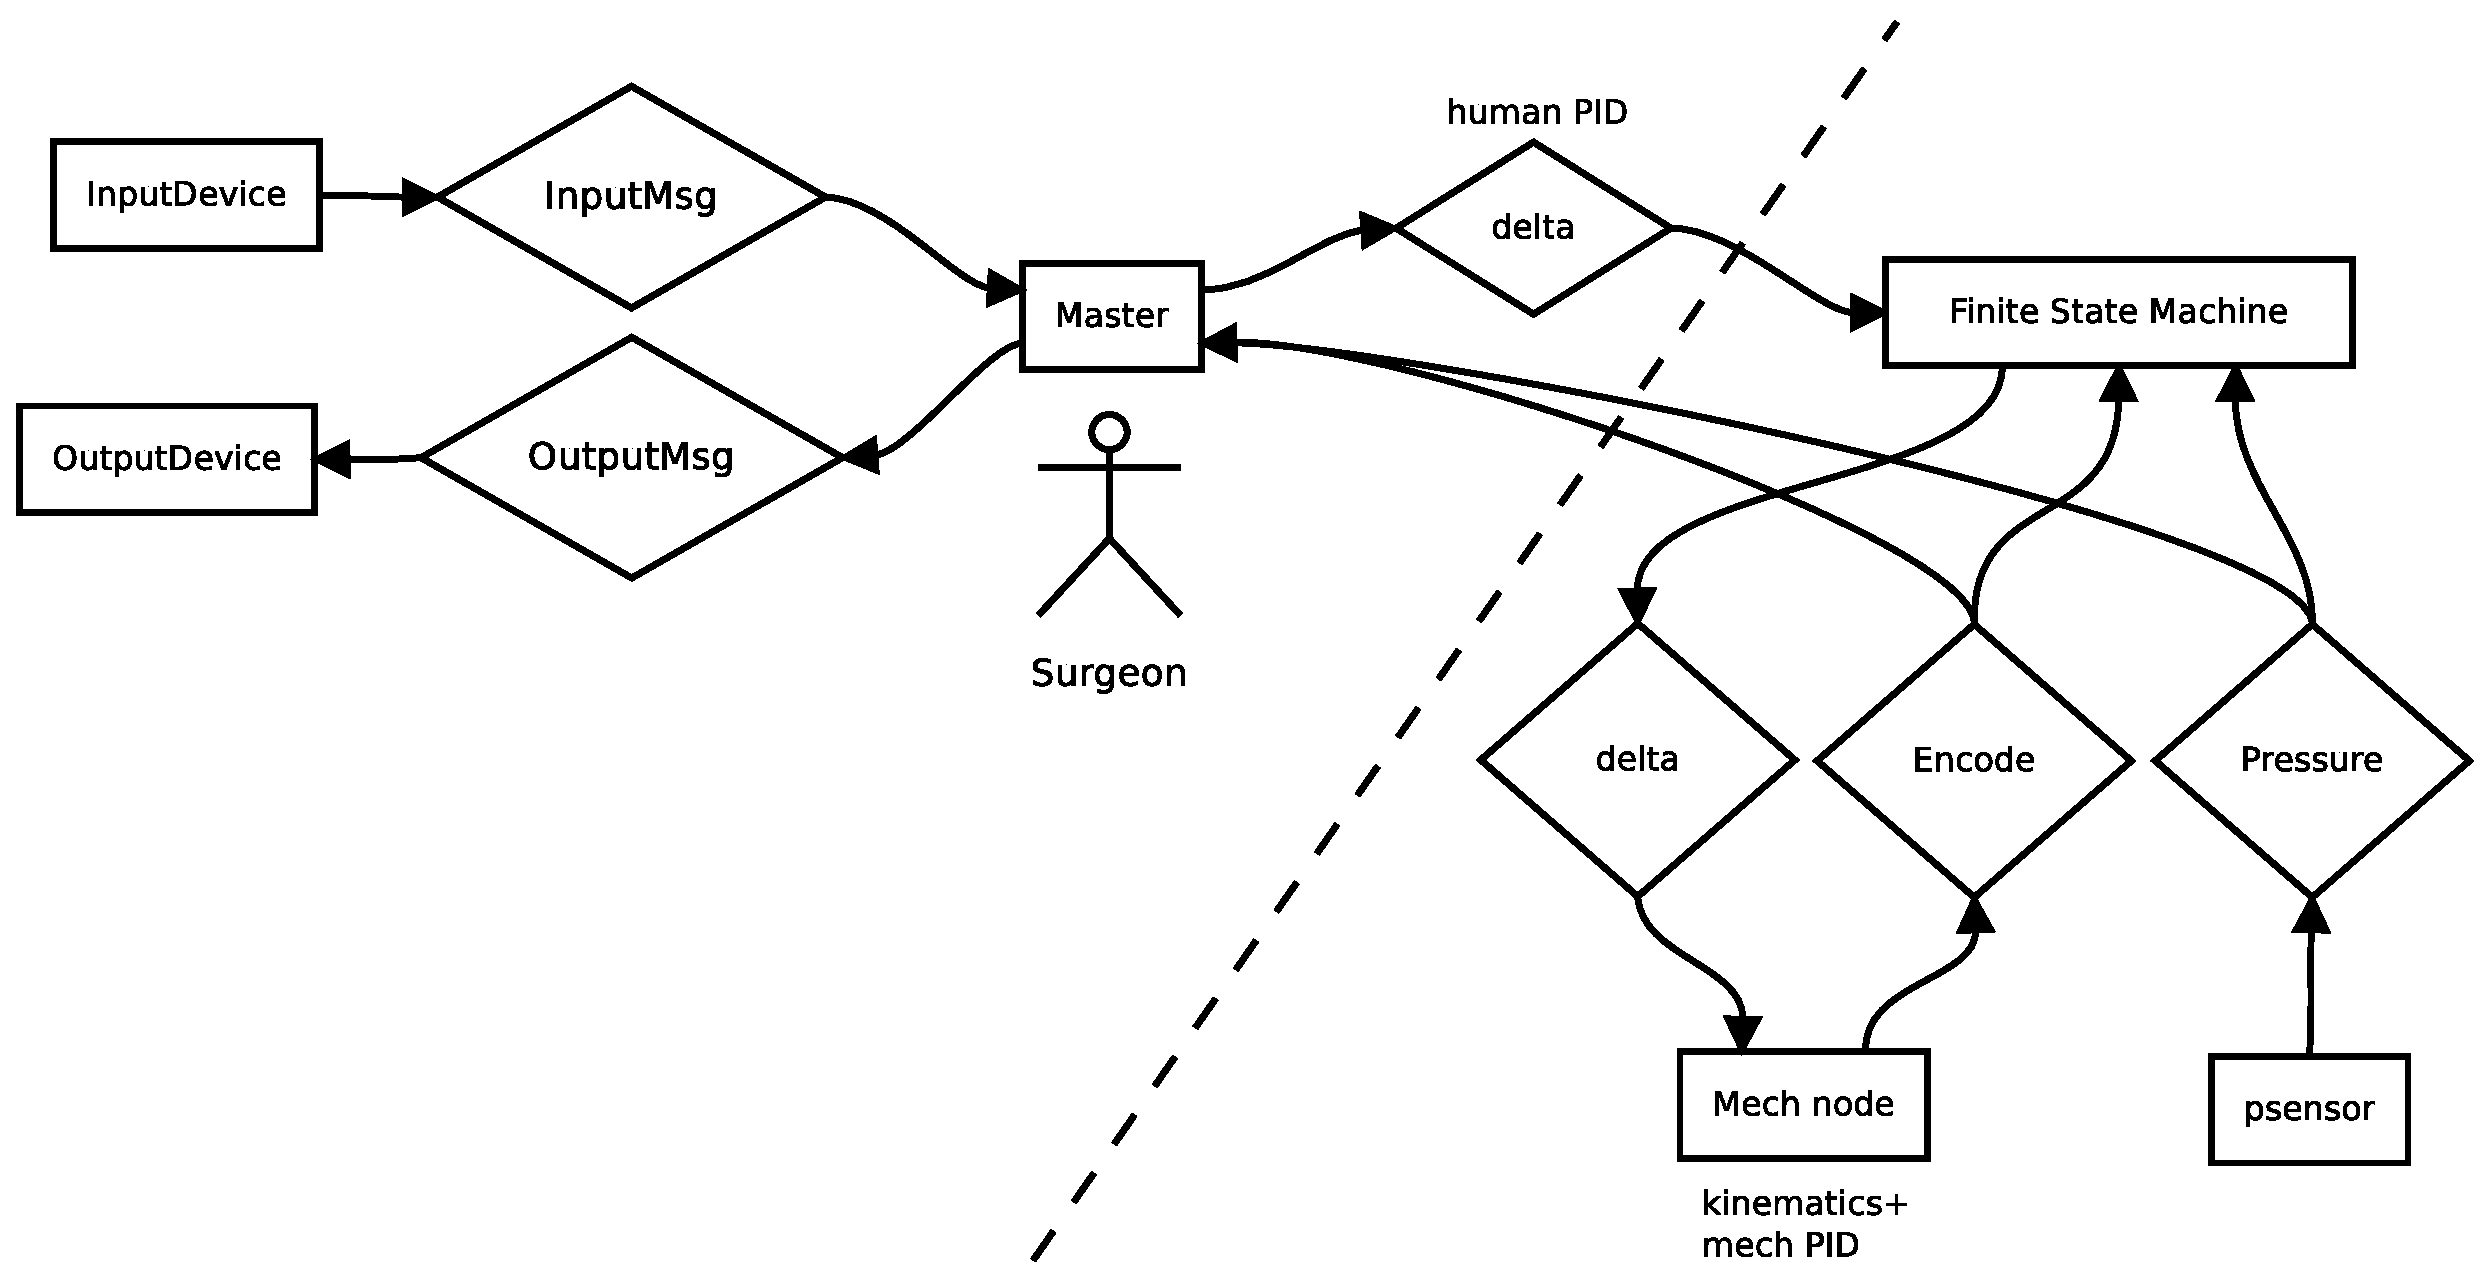
\includegraphics[width=1.0\textwidth]{ros_high_level_v2.eps}
  \end{center}
  \caption{Proposed ROS network for the Raven II. Everything to the
    left of the dashed line is \emph{master}, and everything to the
    right is \emph{slave}. Squares represent ROS nodes, diamonds
    represent ROS topics for passing messages.}
  \label{fig:ros_network}
\end{figure*}

Our top-level design of the ROS network replaces the \emph{networking}
thread, \emph{console I/O} thread, and the entire master side with ROS
components. The square Mech node in Figure~\ref{fig:ros_network}
encasulates most of the existing raven code, including all of the code
responsible for gravity compensation, inverse kinematics, PID control,
and USB I/O. Our ROS network defines a standard interface between the
InputDevice node and the Master node, which would make implementing
new input devices straightforward---adding Wii Remote support or
LapaRobot support to the Raven should be straightforward since it
would not require knowledge of any part of the ROS network beyond its
interface with the Master node.

\subsection{Master: Generic Control}

BRL hard-coded the control side as part of the Raven-II system so that
the control device can only be the Sensable Phantom Omni. Although the
Phantom Omni is a widely used haptic device for medical simulation and
training~\cite{2}, such a constraint would be a limiting factor for projects
involving other types of controllers. In our reimplementation, the
control node is contained within an independent ROS package called
\emph{raven control}. It interacts with the finite state machine in
\emph{raven fsm} through the ROS messaging system, as shown in
Figure~\ref{fig:control_diagram}.

\begin{figure}[h]
  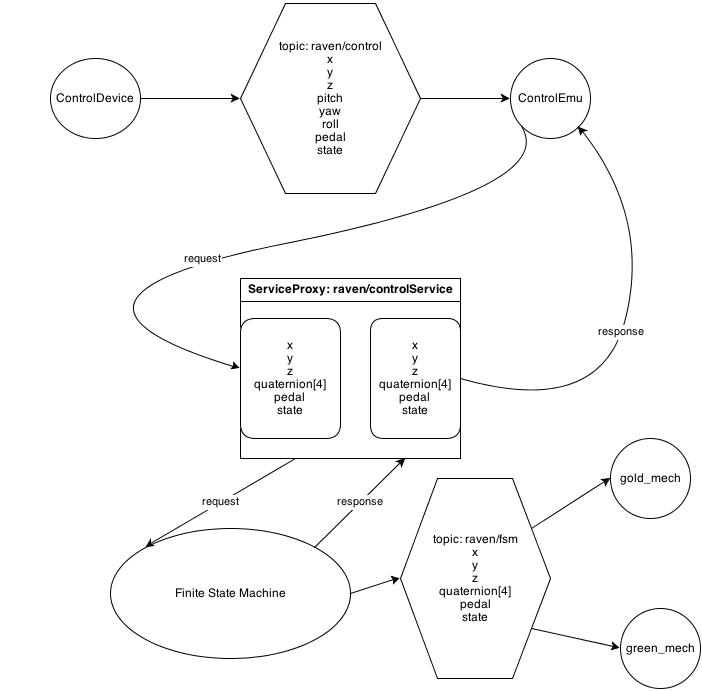
\includegraphics[width=1.0\columnwidth]{ControlDiagram.jpg}
  \caption{Controller-FSM Messaging}
  \label{fig:control_diagram}
\end{figure}

The \emph{ControlDevice} node represents the actual control device on
the user end (e.g. the Phantom Omni). When the user triggers a control
event, \emph{ControlDevice} publishes the message \{x, y, z, pitch,
yaw, roll, pedal, state\} to the topic \emph{raven/control}. On the
subscriber end, \emph{ControlEmu} transforms the values of pitch, yaw
and roll into a quaternion orientation required by
\emph{raven\_mech}. The communication between \emph{ControlEmu} and
the finite state machine is established through a ROS
service\footnote{ROS Services provides a request/reply messaging
  interface between two nodes}. \emph{ControlEmu} sends a request to
the service proxy which the finite state machine (FSM in short)
listens to. Once a control request is received, the FSM formulates a
message object and sends it to the topic \emph{raven/fsm} subscribed
by the arm nodes (the arms are labeled "green" and "gold
respectively"). Once the arms are ready for next control event, the
FSM evaluates the situation and accordingly sends back a response to
\emph{ControlEmu}. \emph{ControlEmu} then issues a new request based
on the previous response.

Compared to the BRL's implementation, our implementation allows
generic control devices besides the Phantom Omni. The tested working
devices are keyboards, PlayStation3 controllers and generic PC game
controllers. Due to the incompleteness of the development, a control
device node needs to be manually added following the template in
Figure~\ref{fig:control_device_template}.

\begin{figure}[h!]
  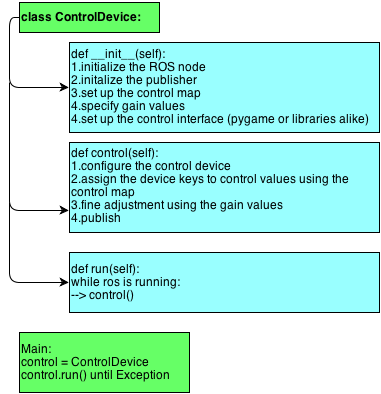
\includegraphics[width=1.0\columnwidth]{ControlDeviceTemplate.png}
  \caption{Control Device Python Template}
  \label{fig:control_device_template}
\end{figure}

Eventually users will be able to add and configure control devices
through either a \emph{control.xml} file or a GTK
interface\footnote{GTK is a programming toolkit for creating graphical
  user interfaces}. The proper control nodes will be generated based
on the user input.

\subsection{Slave: Finite State Machine}

The finite state machine serves as a high-level commander of the
Raven-II system. It's in charge of the state estimation and
transition. Figure~\ref{fig:fsm_workflow} shows the work flow of the FSM.

\begin{figure}[h]
  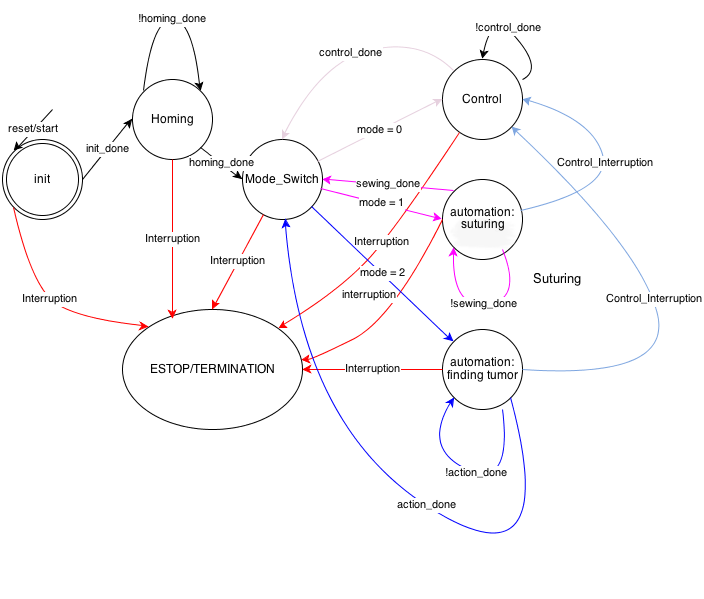
\includegraphics[width=1.0\columnwidth]{FSM.png}
  \caption{FSM Work Flow}
  \label{fig:fsm_workflow}
\end{figure}

After initialization, the FSM starts inspecting \emph{raven\_mech}'s
homing action until it's done. The \texttt{Mode\_Switch} state is
where major estimation and transitions happen. Based on the user
input, the FSM transits to the corresponding state (control, suturing
automation, tumor tracking, etc). The current implementation leaves
room for more modes in the future development. Among all the modes,
``Control'' has the highest priority. Any other modes can be
interrupted by the user control. This is a rather naive implementation
mainly for testing and is subject to change. Among all the states,
\texttt{ESTOP/TERMINATION} has the highest priority. The FSM goes to
this state once there is an emergency interruption. The FSM would then
save the current state record and properly stop the Raven-II
system. The FSM is also designed to communicate with external ROS
nodes. Essentially modes can hand work to ROS nodes and collect status
for progress through services. One example is the controller-FSM
messaging mentioned in the ``Generic Control'' section. If the
``Control'' mode is active, the FSM communicates with
\emph{ControlEmu} through a service, gives \emph{raven\_mech} orders
through messages and reports to \texttt{Mode\_Switch} for state
estimation.

\subsection{Slave: Mech}

Here is where the remainder of the original code can be found. All the
subroutines for handling low-level, Raven-specific components are
currently being encapsulated in a ``black box'' helper library. These
are things that \emph{could} be replaced with ROS parts, but doing so
may not stricty give us an advantage. Some of these components are
listed below:

\begin{itemize}
  \item Code for handling USB I/O. This is where the the code
    interfaces directly with the Raven's hardware controller.

  \item Code for handling Raven-specific arm kinematics. This code is
    derived from a precise mathematical model of the Raven II arm
    design.

  \item Code for PID control and gravity compensation. This code is
    used for dynamically obtaining the desired pose while the arm is
    constantly subject to external forces.
\end{itemize}
 
\section{Results and Conclusion}

Our team has made progress towards total ROS integration taking
several components of the original system and separating them into ROS
packages with clearly defined interfaces. Creating a functional ROS
network was a trivial task, but understanding the original code and
determining the dependencies between each conceptual component was
very time consuming. At the very beginning, the entire code was a big
``black box'', but now that we have broken it into smaller parts and
reduced the size of the original ``black box'', a ROS programmer can
iterate on our work without needing to learn special details of the
robot.

%% {\footnotesize \bibliographystyle{acm}
%% \bibliography{../common/bibliography}}
\twocolumn[
\begin{@twocolumnfalse}
\begin{thebibliography}{9}
\bibitem{}

  \textit{Raven: A Surgical Robot System for Open and Minimally
    Invasive Surgery}, BioRobotics Laboratory, University of
  Washington. \texttt{<http://ee.washington.edu/laboratory/node/26>}

\bibitem{2}

  \textit{The Geomagics Touch Haptic Device},
  \texttt{<http://geomagic.com/en/products/phantom-omni/overview>}

\end{thebibliography}
\end{@twocolumnfalse}
]

%% \theendnotes

\end{document}
